% \setchapterpreamble[u]{\margintoc}
\chapter{Pattern Matching}
\labch{regex}

\section{Introduction}

We have been creating files and directories for a while now,
and we have often required to search for files or directories
in a directory. Till now we used to use the \lstinline|ls| command
to list out all the files in a directory and then check if the
file we are looking for is present in the list or not. This
works fine when the number of files is less, but when the number
of files is large, this method becomes cumbersome. This is where
we can use pattern matching to search for files or directories
or even text in a file.

You would have also used the popular \lstinline|Ctrl+F| shortcut
on most text editors or browsers to search for text in a file
or on a webpage. This is also an example of pattern matching.

\section{Globs and Wildcards}

The simplest form of pattern matching is using globs for filename
expansion. Globs are used to match filenames in the shell.

\begin{definition}[Glob]
A glob is a pattern-matching mechanism used for filename expansion in the shell.
The term "glob" represents the concept of matching patterns globally or
expansively across multiple filenames or paths.
\end{definition}

In bash, we can use the following wildcards to match filenames:

\begin{itemize}
    \item \lstinline|*| - Matches zero or more characters.
    \item \lstinline|?| - Matches exactly one character.
    \item \lstinline|[abc]| - Matches any one of the characters within the square brackets.
    \item \lstinline|[a-z]| - Matches any one of the characters in the range.
    \item \lstinline|[!abc]| - Matches any character except the ones within the square brackets.
\end{itemize}

Let us explore these in detail.

\marginnote{
  Try to guess the output of each of the command before seeing the output.
  If you get an output different from what you expected, try to understand why.
}

\begin{lstlisting}[language=bash]
$ touch abc bbc zbc aac ab
$ ls -1
aac
ab
abc
bbc
zbc
$ echo a*
aac ab abc
$ echo a?
ab
$ echo ?bc
abc bbc zbc
$ echo [ab]bc
abc bbc
$ echo [az]bc
abc zbc
$ echo [a-z]bc
abc bbc zbc
$ echo [!ab]bc
zbc
$ echo [!z]bc
abc bbc
$ echo [!x-z]?c
aac abc bbc
\end{lstlisting}

Shell globs only work with files and directories in the current directory.
The glob expansion to sorted list of valid files in the current directory
is done by the shell, and not by the command itself. It is done before the
command is executed. The command thus does not even know that a glob was
used to expand the filenames. To the command, it looks like the user
directly typed the filenames.

A glob always expands to a space separated list of filenames. However, how
the command interprets this list of filenames is up to the command. Some
commands such as \lstinline|ls -1| will print each filename on a new line,
whereas some commands such as \lstinline|echo| will print all filenames on
the same line separated by a space. \lstinline|echo| does not care if the
arguments passed to it are filenames or not. It just prints them as is.

\begin{lstlisting}[language=bash]
$ echo a*
aac ab abc
$ ls -1 a*
aac
ab
abc
$ ls a*
aac  ab  abc
$ wc a*
0 0 0 aac
0 0 0 ab
0 0 0 abc
0 0 0 total
$ stat a*
  File: aac
  Size: 0               Blocks: 0          IO Block: 4096   regular empty file
Device: 8,2     Inode: 4389746     Links: 1
Access: (0644/-rw-r--r--)  Uid: ( 1000/   sayan)   Gid: ( 1001/   sayan)
Access: 2024-07-12 19:10:27.542322238 +0530
Modify: 2024-07-12 19:10:27.542322238 +0530
Change: 2024-07-12 19:10:27.542322238 +0530
 Birth: 2024-07-12 19:10:27.542322238 +0530
  File: ab
  Size: 0               Blocks: 0          IO Block: 4096   regular empty file
Device: 8,2     Inode: 4389748     Links: 1
Access: (0644/-rw-r--r--)  Uid: ( 1000/   sayan)   Gid: ( 1001/   sayan)
Access: 2024-07-12 19:16:10.707221331 +0530
Modify: 2024-07-12 19:16:10.707221331 +0530
Change: 2024-07-12 19:16:10.707221331 +0530
 Birth: 2024-07-12 19:16:10.707221331 +0530
  File: abc
  Size: 0               Blocks: 0          IO Block: 4096   regular empty file
Device: 8,2     Inode: 4389684     Links: 1
Access: (0644/-rw-r--r--)  Uid: ( 1000/   sayan)   Gid: ( 1001/   sayan)
Access: 2024-07-12 19:10:22.055523865 +0530
Modify: 2024-07-12 19:10:22.055523865 +0530
Change: 2024-07-12 19:10:22.055523865 +0530
 Birth: 2024-07-12 19:10:22.055523865 +0530
\end{lstlisting}

As seen above, the globs simply expand to the filenames in the current path
and pass it as arguments to the command. The output of the command depends
on what command it is. The \lstinline|wc| command counts the number of lines,
words, and characters in a file. The \lstinline|stat| command prints out the
metadata of the files. Similarly, we can use the \lstinline|file| command to
print the type of the files. Try it out.

\begin{exercise}
  Go to an \textbf{empty} directory, and run the following command.
  \begin{lstlisting}[language=bash]
  $ expr 5 * 5
  \end{lstlisting}
  Now run the following command.
  \begin{lstlisting}[language=bash]
  $ touch +
  $ expr 5 * 5
  \end{lstlisting}
  Observe the output of the commands.
  Can you explain why the output is different?
\end{exercise}

When using globs in the shell, if a glob does not match any files, it is
passed as is to the command. The command then interprets the glob as a
normal string.

\begin{lstlisting}[language=bash]
$ touch abc bbc
$ ls
abc  bbc
$ echo ?bc
abc bbc
$ echo ?bd
?bd
\end{lstlisting}

As echo does not care if the arguments passed to it are filenames or not,
it simply prints the arguments as is. The \lstinline|ls| command, however,
will not print the filenames if they do not exist and will instead print
to the standard error that the file does not exist. Use this knowledge
to decipher why the above exercise behaves the way it does.

\section{Regular Expressions}

Globs are good enough when we simply want to run some command and pass
it a list of files matching some pattern. However, when we want to
do more complex pattern matching, we need to use regular expressions.

\begin{definition}[Regular Expression]
A regular expression (shortened as regex or regexp), sometimes
referred to as rational expression, is a sequence of characters
that specifies a match pattern in text. Usually such patterns are
used by string-searching algorithms for "find" or "find and replace"
operations on strings, or for input validation. Regular expression
techniques are developed in theoretical computer science and formal
language theory.
\end{definition}

Due to the powerfullness of regular expressions, almost all programming
languages and text processing tools support regular expressions directly.
This makes text processing very easy and powerful, as well as cross-platform.

However, there are multiple flavors of regular expressions, and the syntax
of each flavor may differ slightly. The most common flavors are:

\begin{itemize}
    \item Basic Regular Expressions (BRE)
    \item Extended Regular Expressions (ERE)
    \item Perl-Compatible Regular Expressions (PCRE)
\end{itemize}

These are the regular expressions that are supported by most text processing
utilities in Unix-like systems. These follow the POSIX standard for regular
expressions.
There are also Perl syntax regular expressions,
which are more powerful and flexible, and are supported by the Perl programming
language.
\sidenote{
PCRE and Perl Regex are not the same. PCRE is a library that implements Perl
like regular expressions, but in C. Perl Regex is the regular expression
that is used in the Perl programming language.
More details can be found
\href{https://en.wikipedia.org/wiki/Perl\_Compatible\_Regular\_Expressions}{online}.
}

We will focus on BRE and ERE in this chapter, as these are the most commonly
used flavors in Unix-like systems.

\subsection{Basic Regular Expressions}

Basic Regular Expressions (BRE) are the simplest form of regular expressions.
They are supported by most Unix-like systems and are the default regular
expressions used by most text processing utilities such as \lstinline|grep|,
and \lstinline|sed|.
\sidenote{
  awk uses ERE by default, not BRE.
}

BRE syntax is similar to the glob syntax, but with more power and flexibility.
There are some subtle differences between the two.

The following are the basic regular expressions that can be used in BRE:

\begin{itemize}
  \item \lstinline|a| - Matches the character a.
  \item \lstinline|.| - Matches any single character exactly once.
  \item \lstinline|*| - Matches zero or more occurrences of the previous character.
  \item \lstinline|^| - Matches the null string at the start of a line.
  \item \lstinline|$| - Matches the null string at the end of a line.
  \item \lstinline|[abc]| - Matches any one of the characters within the square brackets.
  \item \lstinline|[a-z]| - Matches any one of the characters in the range, both ends inclusive.
  \item \lstinline|[^abc]| - Matches any character except the ones within the square brackets; the caret symbol has a different meaning when inside the brackets.
  \item \lstinline|\+| - Matches one or more occurrences of the previous character.
  \item \lstinline|\?| - Matches zero or one occurrence of the previous character.
  \item \lstinline|{n}| - Matches exactly n occurrences of the previous character.
  \item \lstinline|{n,}| - Matches n or more occurrences of the previous character.
  \item \lstinline|{n,m}| - Matches n to m occurrences of the previous character.
  \item \lstinline|\| - Escapes a special character such as \lstinline|*|, \lstinline|.|, \lstinline|[|, \lstinline|\|, \lstinline|$|, or \lstinline|^|.
  \item \lstinline/regex1|regex2/ - Matches either regex1 or regex2.
  \item \lstinline|(regex)| - Groups the regex.
    \item \lstinline|\2| - Matches the 2-nd \lstinline|(...)| parenthesized subexpression in the regular expression. This is called a back reference. Subexpressions are implicitly numbered by counting occurrences of \lstinline|(| left-to-right.
  \item \lstinline|\n| - Matches a newline character.
\end{itemize}

\subsection{Character Classes}
A bracket expression is a list of characters enclosed by '[' and ']'. It matches any single character in that list; if the first character of the list is the caret '\textasciicircum', then it matches any character not in the list.
For example, the following regex matches the words 'gray' or 'grey'.

\lstinline|gr[ae]y|

Let's create a small script to test this regex.

\begin{lstlisting}[language=bash]
$ cat regex1.sh
#!/bin/bash
read -r -p "Enter color: " color
if [[ $color =~ gr[ae]y ]]; then
    echo "The color is gray or grey."
else
    echo "The color is not gray or grey."
fi
$ ./regex1.sh
Enter color: gray
The color is gray or grey.
$ ./regex1.sh
Enter color: grey
The color is gray or grey.
$ ./regex1.sh
Enter color: green
The color is not gray or grey.
\end{lstlisting}

\subsubsection{Ranges}

Within a bracket expression, a range expression consists of two characters separated by a hyphen. It matches any single character that sorts between the two characters, inclusive. In the default C locale, the sorting sequence is the native character order; for example, ‘[a-d]’ is equivalent to ‘[abcd]’.
\sidenote{
  There are locales other than the default C locale, such as the en\_US.UTF-8 locale, which sorts and collates characters differently. In the en\_US.UTF-8 locale, the sorting sequence is based on the Unicode code points of the characters and collates characters with accents along with the characters.
}

For example, the following regex matches any lowercase letter.

\lstinline|[a-z]|

Let's create a small script to test this regex.

\begin{lstlisting}[language=bash]
$ cat regex2.sh
#!/bin/bash
read -r -p "Enter a letter: " letter
if [[ $letter =~ [a-z] ]]; then
    echo "The letter is a lowercase letter."
else
    echo "The letter is not a lowercase letter."
fi
$ ./regex2.sh
Enter a letter: a
The letter is a lowercase letter.
$ ./regex2.sh
Enter a letter: A
The letter is not a lowercase letter.
\end{lstlisting}

\subsubsection{Named Character Classes}

There are some predefined character classes which are used often, that can be used in regular expressions. These classes contain a pair of brackets, and should be
present inside a bracket expression. Some of the common character classes are:

\begin{itemize}
  \item \lstinline|[[:alnum:]]| - Alphanumeric characters: \lstinline|[[:alpha:]]| and \lstinline|[[:digit:]]|; in the ‘C’ locale and ASCII character encoding, this is the same as \lstinline|[0-9A-Za-z]|.
  \item \lstinline|[[:alpha:]]| - Alphabetic characters: \lstinline|[[:lower:]]| and \lstinline|[[:upper:]]|; in the ‘C’ locale and ASCII character encoding, this is the same as \lstinline|[A-Za-z]|.
  \item \lstinline|[[:blank:]]| - Blank characters: space and tab.
  \item \lstinline|[[:cntrl:]]| - Control characters. In ASCII, these characters have octal codes 000 through 037, and 177 (DEL). In other character sets, these are the equivalent characters, if any.
  \item \lstinline|[[:digit:]]| - Digits: 0 1 2 3 4 5 6 7 8 9.
  \item \lstinline|[[:graph:]]| - Graphical characters: \lstinline|[[:alnum:]]| and \lstinline|[[:punct:]]|.
  \item \lstinline|[[:lower:]]| - Lower-case letters; in the ‘C’ locale and ASCII character encoding, this is a b c d e f g h i j k l m n o p q r s t u v w x y z.
  \item \lstinline|[[:print:]]| - Printable characters: \lstinline|[[:alnum:]]|, \lstinline|[[:punct:]]|, and space.
  \item \lstinline|[[:punct:]]| - Punctuation characters.
  \item \lstinline|[[:space:]]| - Space characters: in the ‘C’ locale, this is tab, newline, vertical tab, form feed, carriage return, and space.
  \item \lstinline|[[:upper:]]| - Upper-case letters: in the ‘C’ locale and ASCII character encoding, this is A B C D E F G H I J K L M N O P Q R S T U V W X Y Z.
  \item \lstinline|[[:xdigit:]]| - Hexadecimal digits: 0 1 2 3 4 5 6 7 8 9 A B C D E F a b c d e f.
\end{itemize}

These named character classes's expansion depends on the locale. For example, in the en\_US.UTF-8 locale, the \lstinline|[[:lower:]]| class will match all lowercase letters in the Unicode character set, not just the ASCII character set.

It is important to note that these named character classes should be present
inside two square brackets, and not just one. If we use only one square bracket,
it will intepret each character inside the square brackets as a separate character
in the list.

\lstinline|[:digit:]| will match any of the characters \lstinline|d g i t :|.
If a character is repeated in the list, it has no additional effect.

Some characters have different meaning inside the list depending on the
position they are in. For example, the caret symbol \lstinline|^| negates
the entire list if it is the first character in the list, but is matched
literally if it is not the first character in the list.

\begin{itemize}
  \item \lstinline|]| is used to end the list of characters, unless it is the first character in the list, then it is matched literally.
  \item \lstinline|-| is used to specify a range of characters, unless it is the first or last character in the list, then it is matched literally.
  \item \lstinline|^| is used to negate the list of characters if it is the first character in the list, else it is matched literally.
\end{itemize}

Example for \lstinline|]|:
\marginnote{
  From this example, we have started using the \lstinline|grep| command to match
  regex quickly instead of creating a script. We will discuss the \lstinline|grep|
  command in more detail later in this chapter. The \lstinline|-o| flag is used
  to print only the matching part of the line, instead of the entire line.
  If you omit it, and run the command, you will see the entire line that
  has the matching part being printed, however the matching part may still
  be highlighted using color, As it is not possible to highlight the matching
  part in this book, we are using the \lstinline|-o| flag to print only the
  matching part.
}
\begin{lstlisting}[language=bash]
$ echo "match square brackets [ and ]" | grep -o '[mb]'
m
b
$ echo "match square brackets [ and ]" | grep -o '[]mb]'
m
b
]
\end{lstlisting}

Example for \lstinline|-|:
\marginnote{
  Observe how putting the hyphen at the start of the list makes it match
  the hyphen literally, whereas putting it in the middle makes it match
  a range of characters.
}
\begin{lstlisting}[language=bash]
$ echo "ranges are separated by hyphens like - " | grep -o '[a-c]'
a
a
a
a
b
$ echo "ranges are separated by hyphens like - " | grep -o '[-a-c]'
a
a
a
a
b
-
\end{lstlisting}

\marginnote{
  The caret symbol \lstinline|^| is used to negate the list of characters
  if it is the first character in the list, else it is matched literally.
  First case will match any character except \lstinline|l|, \lstinline|i|,
  \lstinline|n|, \lstinline|e|, and the second case will match only the
  characters \lstinline|l|, \lstinline|i|, \lstinline|n|, \lstinline|e|
  and the caret symbol \lstinline|^|.
}
Example for \lstinline|^|:
\begin{lstlisting}[language=bash]
$ echo "this is a ^line^" | grep -o '[^line]'
t
h
s

s

a

^
^
$ echo "this is a ^line^" | grep -o '[line^]'
i
i
^
l
i
n
e
^
\end{lstlisting}

\subsubsection{Collating Symbols}

A collating symbol is a single-character collating element enclosed in ‘[.’ and ‘.]’. It stands for a collating element that collates with a single character, as if the character were a separate character in the POSIX locale’s collation order.
Collating symbols are typically used when a digraph is treated like a single character in a language. They are an element of the POSIX regular expression specification, and are not widely supported.

For example, the Welsh alphabet
\sidenote{
  Read more about the Welsh alphabet
  \href{https://en.wikipedia.org/wiki/Welsh\_orthography}{here}.
}
has a number of digraphs that are treated as a single letter (marked with a * below)

\begin{lstlisting}
a b c ch d dd e f ff g ng h i j l ll m n o p ph r rh s t th u w y
       *           *    *          *          *    *      *
\end{lstlisting}

Assuming the locale file defines it
\sidenote{
  a collating symbol will only work if it is defined in the current locale
}
, the collating symbol
\lstinline|[[.ng.]]|
is treated like a single character. Likewise, a single character expression like . or
\lstinline|[^a]|
will also match "ff" or "th." This also affects sorting, so that
\lstinline|[p-t]|
will include the digraphs "ph" and "rh" in addition to the expected single letters.

A collating symbol represents a set of characters which are considered as a single unit for collating (sorting) purposes; for example, "ch"/"Ch" or "ss" (these are only valid in locales which define them);

\subsubsection{Equivalence Classes}

An equivalence class groups characters which are equivalent for collating purposes; for example, "a" and "à" (and other accented variants).

\lstinline|[[=a=]]| is an equivalence class that matches the character "a" and all its accented variants, such as aªáàâãäå, etc.

Collating symbols and equivalence classes are used in locale definitions to encode complex ordering information and are not implemented in some regular expression engines. We will not discuss these in depth.

\subsubsection{Escape Sequences}

Along with the named character classes, there are some escape sequences that can be used in regular expressions. These are:

\begin{itemize}
  \item \lstinline|\b| - Matches a word boundary; that is it matches if the character to the left is a “word” character and the character to the right is a “non-word” character, or vice-versa. It does not match any character, but matches the empty string that marks the word delimition.
  \item \lstinline|\B| - Matches a non-word boundary; that is it matches if the characters on both sides are either “word” characters or “non-word” characters.
  \item \lstinline|\<| - Matches the start of a word only.
  \item \lstinline|\>| - Matches the end of a word only.
  \item \lstinline|\d| - Matches a digit character. Equivalent to \lstinline|[0-9]|.
  \item \lstinline|\D| - Matches a non-digit character. Equivalent to \lstinline|[^0-9]|.
  \item \lstinline|\s| - Matches a whitespace character. Equivalent to \lstinline|[[:space:]]|.
  \item \lstinline|\S| - Matches a non-whitespace character. Equivalent to \lstinline|[^[:space:]]|.
  \item \lstinline|\w| - Matches a word character. Equivalent to \lstinline|[[:alnum:]_]|.
  \item \lstinline|\W| - Matches a non-word character. Equivalent to \lstinline|[^[:alnum:]_]|.
  \item \lstinline|\`| - Matches the start of pattern space if multiline mode is enabled.
  \item \lstinline|\'| - Matches the end of pattern space if multiline mode is enabled.
\end{itemize}

Other than these, other escape characters are present to match special non-graphical characters such as newline, tab, etc. These are GNU extensions and are not defined in the original POSIX standard.

\begin{itemize}
  \item \lstinline|\a| - Matches the alert character (ASCII 7).
  \item \lstinline|\f| - Matches the form feed character (ASCII 12).
  \item \lstinline|\n| - Matches the newline character (ASCII 10).
  \item \lstinline|\r| - Matches the carriage return character (ASCII 13).
  \item \lstinline|\t| - Matches the tab character (ASCII 9).
  \item \lstinline|\v| - Matches the vertical tab character (ASCII 11).
  \item \lstinline|\0| - Matches the null character (ASCII 0).
  \item \lstinline|\cx| - Matches the control character x. For example, \lstinline|\cM| matches the carriage return character. This converts lowercases to uppercase then flips the bit-6 of the character.
  \item \lstinline|\xxx| - Matches the character with the hex value $xx$.
  \item \lstinline|\oxxx| - Matches the character with the octal value $xxx$.
  \item \lstinline|\dxxx| - Matches the character with the decimal value $xxx$.
\end{itemize}

You can also read more about the locale issues in regex
\href{https://www.gnu.org/software/sed/manual/html\_node/Locale-Considerations.html#Locale-Considerations}{here}.

\subsection{Anchors}

Anchors are used to match a position in the text, rather than a character. The following are the anchors that can be used in regular expressions:

\begin{itemize}
  \item \lstinline|^| - Matches the start of a line.
  \item \lstinline|$| - Matches the end of a line.
  \item \lstinline|\b| - Matches a word boundary.
  \item \lstinline|\B| - Matches a non-word boundary.
  \item \lstinline|\<| - Matches the start of a word.
  \item \lstinline|\>| - Matches the end of a word.
  \item \lstinline|\`| - Matches the start of the pattern space if multiline mode is enabled.
    \item \lstinline|\'| - Matches the end of the pattern space if multiline mode is enabled.
\end{itemize}

These anchors are used to match the position in the text, rather than the character. For example, the regex \lstinline|^a| will match the character \lstinline|a| only if it is at the start of the line. It does not match any other character other than the \lstinline|a|. However, if there are not \lstinline|a| present at the start of the line, then nothing is matched at all.

\marginnote{
  \lstinline|xxd| is a command that is used to convert a file to a hex dump. It is used here to show the output in a more readable format.
  $61$ is the hex value of the character \lstinline|a|.
  $0a$ is the hex value of the newline character.
  The lack of output in the second case means that nothing is matched, and
  no bytes are output.
}
\begin{lstlisting}[language=bash]
$ echo "apple" | grep -o '^a'
a
$ echo "apple" | grep -o '^a' | xxd
00000000: 610a                                     a.
$ echo "banana" | grep -o '^a'
$ echo "banana" | grep -o '^a' | xxd
\end{lstlisting}

The anchors
\lstinline|^|,
\lstinline|$|, and
\lstinline|\b|
are very useful in most of the text processing tasks. The \lstinline|^| and
\lstinline|$| when used together can match the entire line, meaning that the
pattern between them is not matched if it is a substring of the line; it
only matches if the pattern is the entire line. The \lstinline|\b| is used
to surround the pattern if we want to match the pattern as a word, and not
as substring of a word.

\begin{lstlisting}[language=bash]
$ echo "apple" | grep -o '^apple$'
apple
$ echo "apple is great" | grep -o '^apple$'
$ echo "apple is great" | grep -o '\bapple\b'
apple
$ echo "i like pineapple" | grep -o '\bapple\b'
\end{lstlisting}

Observe that even though we are using the \lstinline|-o| flag, the entire word
is printed in a single line. This is because the \lstinline|-o| flag prints
only the matches and prints them on separate lines. However, unlike the previous
cases where we were using character lists, here the entire word is a single match,
and thus is printed on a single line.

\subsection{Quantifiers}

Quantifiers are used to match a character or a group of characters multiple times.
This is useful if we do not know the exact number of times a character or group of characters will be repeated or its length. Paired with a character list, it makes
regex very powerful and able to match any arbitrary pattern.

The following are the quantifiers that can be used in regular expressions:

\begin{itemize}
  \item \lstinline|*| - Matches zero or more occurrences of the previous character.
  \item \lstinline|\+| - Matches one or more occurrences of the previous character.
  \item \lstinline|\?| - Matches zero or one occurrence of the previous character.
  \item \lstinline|{n}| - Matches exactly n occurrences of the previous character.
  \item \lstinline|{n,}| - Matches n or more occurrences of the previous character.
  \item \lstinline|{,n}| - Matches n or less occurrences of the previous character.
  \item \lstinline|{n,m}| - Matches n to m occurrences of the previous character, both ends inclusive.
\end{itemize}

Note that \lstinline|+| and \lstinline|?| are not part of the BRE standard, but are part of the ERE standard. However, most text processing utilities support them in BRE mode as well if escaped.

\begin{lstlisting}[language=bash]
$ echo -n "aaaaaaaaaaaaaa" | wc -c # there are 14 a's
14
$ echo "aaaaaaaaaaaaaa" | grep -E "a{4}" -o # the first 12 a's are matched in groups of four
aaaa
aaaa
aaaa
$ echo "aaaaaaaaaaaaaa" | grep -E "a{4,}" -o # entire string is matched
aaaaaaaaaaaaaa
$ echo "aaaaaaaaaaaaaa" | grep -E "a{4,5}" -o # maximal matching, first 10 a's are matched as groups of 5, then the last 4 a's are matched as group of four.
aaaaa
aaaaa
aaaa
$ echo "aaaaaaaaaaaaaa" | grep -E "a{,5}" -o
aaaaa
aaaaa
aaaa
\end{lstlisting}

\marginnote{
  Here we are using the \lstinline|-E| flag to enable ERE mode in \lstinline|grep|.
  If we are using the default BRE mode, we need to escape the \lstinline|+|, \lstinline|?|, \lstinline|\{|, and \lstinline|\}|, \lstinline|(|, \lstinline|)|, \lstinline/|/ characters to use them.
}

Let us also see how the \lstinline|*|, \lstinline|+| and \lstinline|?| quantifiers work.

\begin{lstlisting}[language=bash]
$ echo "There are there main quantifiers, which are asterisk (*), plus (+), and eroteme (?)." | grep "[^aeiou][aeiou]*" -o
T
he
re
 a
re

t
he
re

mai
n

qua
n
ti
fie
r
s
,

w
hi
c
h
 a
re
 a
s
te
ri
s
k

(
*
)
,

p
lu
s

(
+
)
,
 a
n
d
 e
ro
te
me

(
?
)
.
\end{lstlisting}

This shows that the asterisk quantifier matches zero or more occurrences of the previous character, here we are matching for any pattern which does not start with a vowel and has zero or more vowels after it, thus the matching can keep on growing as long as there are consequtive vowels. As soon as a non-vowel is present, the previous match ends and a new match starts.

Now compare and constrast the previous output to the next output using the plus quantifier. The lines with only a single character (non-vowel) will no longer be present.

\begin{lstlisting}[language=bash]
$ echo "There are there main quantifiers, which are asterisk (*), plus (+), and eroteme (?)." | grep "[^aeiou][aeiou]\+" -o
he
re
 a
re
he
re
mai
qua
ti
fie
hi
 a
re
 a
te
ri
lu
 a
 e
ro
te
me
\end{lstlisting}

Finally, observe how using the eroteme quantifier will bring back the single character lines, but remove the lines with more than a vowel.

\begin{lstlisting}[language=bash]
$ echo "There are there main quantifiers, which are asterisk (*), plus (+), and eroteme (?)." | grep "[^aeiou][aeiou]\?" -o
T
he
re
 a
re

t
he
re

ma
n

qu
n
ti
fi
r
s
,

w
hi
c
h
 a
re
 a
s
te
ri
s
k

(
*
)
,

p
lu
s

(
+
)
,
 a
n
d
 e
ro
te
me

(
?
)
.
\end{lstlisting}

When mixed with character lists, quantifiers can be used to match any arbitrary pattern. This makes regular expressions very powerful and flexible.

\begin{lstlisting}[language=bash]
$ echo "sometimes (not always) we use parentheses (round brackets) to clarify some part of a sentence (or phrase)." | grep "([^)]\+)" -o
(not always)
(round brackets)
(or phrase)
\end{lstlisting}

Observe how \lstinline|([^)]\+)| matches any pattern that starts with an opening parenthesis, followed by one or more characters that are not a closing parenthesis, and ends with a closing parenthesis. This lets us all of the bracketed parts of a sentence, without knowing how many such brackets exist, or what is the length of each expression. This is pretty powerful, and can be used in similar situations, such as extracting text from HTML tags
\sidenote{
  Regular Expressions can only match regular languages, and not context-free languages, context-sensitive languages, or unrestricted languages. This means that they cannot be used to parse HTML or XML files. However, for simple tasks such as extracting text from tags, regular expressions can be used.
  To explore community lore on this topic, see
  \href{https://stackoverflow.com/questions/1732348/regex-match-open-tags-except-xhtml-self-contained-tags}{this stackoverflow answer}.
  To learn more about the theoretical aspects of regular expressions, see
  \href{https://www.geeksforgeeks.org/chomsky-hierarchy-in-theory-of-computation/}{Chomsky Hierarchy in Theory of Computation}.
}
JSON strings, etc.

\subsection{Alternation}

Alternation is used to match one of the multiple patterns. It is used to match multiple patterns in a single regex. The syntax for alternation is \lstinline:regex1|regex2:. The regex will match if either \lstinline|regex1| or \lstinline|regex2| is matched.

Alternation in BRE needs to be escaped, as it is not part of the standard. However, most text processing utilities support it in BRE mode if escaped.

\begin{lstlisting}[language=bash]
$ echo -e "this line starts with t\nand this starts with a\nwhereas this line starts with w" | grep '^t'
this line starts with t
$ echo -e "this line starts with t\nand this starts with a\nwhereas this line starts with w" | grep '^t\|^a'
this line starts with t
and this starts with a
\end{lstlisting}

As seen above, the regex \lstinline:^t\|^a: matches any line that starts with either \lstinline|t| or \lstinline|a|. This is very useful when we want to match multiple patterns in a single regex. Note that we have to mention the start of line anchor both times, this is because
alternation has the lowest precedence, and thus the start of line anchor is not shared between the two patterns.

Let us now see a more complex example of alternation similar to previous example of brackets.

\begin{lstlisting}[language=bash]
$ echo "sometimes (not always) we use parentheses (round brackets) or brackets [square brackets] to clarify some part of a sentence (or phrase)." | grep "([^)]\+)\|\[[^\]\+\]" -o
(not always)
(round brackets)
[square brackets]
(or phrase)
\end{lstlisting}

Here we are matching phrases inside round OR square brackets.
Observe a few things here:

\begin{enumerate}
  \item We need to escape the alternation operator \lstinline:|: as it is not part of the BRE standard.
  \item We need to escape the square brackets \lstinline|[]| when we want it to match literally as they have special meaning in regex.
  \item We need to escape the plus quantifier \lstinline|+| as it is not part of the BRE standard.
\end{enumerate}

\subsection{Grouping}

Grouping is used to group multiple characters or patterns together. This is useful when we want to apply a quantifier to multiple characters or patterns. The syntax for grouping is \lstinline|(regex)|. The regex will match if the pattern inside the parentheses is matched. The parenthesis will not be matched. However, grouping is not present unescaped in BRE, so if we want to match literal parenthesis then we use \lstinline|(regex)|, and if we want to group the regex without matching the parenthesis, then we use \lstinline|(regex)|.

Let's revisit one of the earlier examples of alternation, and group the patterns inside the alternation.

\begin{lstlisting}[language=bash]
$ echo -e "this line starts with t\nand this starts with a\nwhereas this line starts with w" | grep '^t\|^a'
this line starts with t
and this starts with a
$ echo -e "this line starts with t\nand this starts with a\nwhereas this line starts with w" | grep '^\(t\|a\)'
this line starts with t
and this starts with a
\end{lstlisting}

As evident from above, both the grouped and ungrouped regexes match the same lines.
But in the grouped version, we do not have to repeat the start of line anchor, and the regex is more readable.
Also, grouping is useful when we want to apply a quantifier to the entire group.


\marginnote{
  Notice the subtly different way of providing the string to the stdin of the \lstinline|grep| command. We have covered here-strings earler.
}
\begin{lstlisting}[language=bash]
$ grep -E "([b-d]|[f-h]|[j-n]|[p-t]|[v-z]){2}" -o <<< "this is a sentence"
th
nt
nc
\end{lstlisting}

In this example, we are matching any two consecutive characters that are consonants.
Here we are not matching \textbf{not vowels}, rather we are explicitly matching consonants which are lowercase. Thus this will not match spaces, digits, or punctuations.
There is no direct way to match consonants in BRE, so we have to list them explicitly and chain them using alternations.
However, if we want to match two consonants consequtively we do not have to list the entire pattern again, we can simply group it and apply the \lstinline|{n}| quantifier on it.

The biggest use-case of grouping is to refer to the matched group later in the regex. This is called backreferencing, and is very useful when we want to match a pattern that is repeated later in the text.

\begin{lstlisting}[language=bash]
$ grep -E "([b-d]|[f-h]|[j-n]|[p-t]|[v-z]){2}" -o <<< "this is an attached sentence"
th
tt
ch
nt
nc
\end{lstlisting}

Observe in this similar example, where the input string now has the word \textbf{attached} in it. One of the matched pattern is \lstinline|tt|. But if we want to \textbf{only} list those consonants groups that use the same consonant, like \lstinline|tt|? Then we require to use \textbf{backreferencing}.

\subsection{Backreferences}

Backreferences are used to refer to a previously matched group in the regex. This is useful when we want to match a pattern that is repeated later in the text. The syntax for backreferencing is \lstinline|\n|, where \lstinline|n| is the number of the group that we want to refer to. The group is implicitly numbered by counting occurrences of \lstinline|(...)| left-to-right.

To accomplish the previous example, we use the backreference \lstinline|\1| to match only the same consonant, and not repeat the match using \lstinline|{n}|.

\begin{lstlisting}[language=bash]
$ grep -E "([b-d]|[f-h]|[j-n]|[p-t]|[v-z])\1" -o <<< "this is an attached sentence"
tt
\end{lstlisting}

Backreferences are also useful in tools such as \lstinline|sed| and \lstinline|awk| where we can replace the string with another string and can use the matched group and in the replacement string.

For example, if we want to make the first letter of either \lstinline|apple| or \lstinline|banana| uppercase, we can use the following command.


\begin{lstlisting}[language=bash]
$ echo "apple & banana" | sed -E 's/\<([ab])/\U\1/g'
Apple & Banana
\end{lstlisting}

Here we are using the \lstinline|sed| command to replace the matched pattern with the uppercase version of the first character. The \lstinline|\1| is used to refer to the first matched group, which is the first character of the word.
The syntax of sed is \lstinline|s/pattern/replacement/flags|, where \lstinline|pattern| is the regex to match, \lstinline|replacement| is the string to replace the matched pattern with, and \lstinline|flags| are the flags to apply to the regex.
The replacement string has to be a string, and not a regex, however, we can use backreferences in the replacement string.
The \lstinline|\U| is used to convert the matched group to uppercase.
The \lstinline|g| flag is used to replace all occurrences of the pattern in the line.
The \lstinline|\<| is used to match the start of the word, otherwise the \lstinline|a| inside \lstinline|banana| will also be capitalized.
We will cover \lstinline|sed| in details in later chapters.

Let us use backreferences to find three letter palindromes in a string.
You should have a dictionary of words in \lstinline|/usr/share/dict/words|.
\sidenote{
  If your distribution does not have the \lstinline|/usr/share/dict/words| file, you can download it from
  \href{https://github.com/dwyl/english-words/blob/master/words.txt}{here}.
}

\marginnote{
  Here we are preprocessing the dictionary to convert all the words to lowercase using the \lstinline|tr| command. Then we are passing the output of \lstinline|tr| to \lstinline|grep| to find the lines that match the pattern
  \lstinline|^([a-z])[a-z]\1$|. This pattern matches any three letter palindrome. The \lstinline|^| and \lstinline|$| are used to match the start and end of the line respectively.
  The \lstinline|([a-z])| is used to match any lowercase letter, and the \lstinline|\1| is used to match the same letter as the first matched group. This is used to match the palindrome.
  Finally, as the output is too large, we are using the \lstinline|tail| command to print only the last 50 lines.
  We have used process substitution as well as pipes in this, so the flow of data is not strictly left to right. Revise the previous chapters and try to understand how the data is flowing.
  What difference would it make if we replaced \lstinline|<(tr| with \lstinline|< <(tr|, in the internal workings and the output of the command?
}
\begin{lstlisting}[language=bash]
$ grep -E "^([a-z])[a-z]\1$" <(tr 'A-Z' 'a-z' < /usr/share/dict/words ) | tail -n30
rsr
rtr
sas
sbs
scs
sds
ses
sis
sls
sms
sos
sps
srs
sss
sts
sus
svs
sws
sxs
tat
tct
tet
tft
tgt
tit
tyt
tkt
tnt
tot
tpt
trt
tst
tut
twt
txt
ulu
umu
upu
uru
usu
utu
vav
viv
waw
wnw
wow
wsw
xix
xxx
zzz
\end{lstlisting}

\section{Extended Regular Expressions}

Throughout the chapter, we have noticed that some regex syntax are not really
supported in BRE standard, and to use them in most text processing applications when using BRE, we have to escape them. Explicitly, the characters that are not supported in BRE but are supported in ERE are as follows.

\begin{itemize}
  \item \lstinline|+| - In BRE, it would match the literal plus sign if not escaped. Otherwise it is a quantifier of the previous character or group, making it one or more.
  \item \lstinline|?| - In BRE, it would match the literal eroteme sign if not escaped. Otherwise it is a quantifier of the previous character or group, making it zero or one, not more.
  \item \lstinline|(| and \lstinline|)| - The parenthesis match literal parenthesis in the data in BRE if unescaped, otherwise are used to group regular expressions.
  \item \lstinline|{| and \lstinline|}| - The curly braces match literal curly braces in the data in BRE if unescaped, otherwise are used to specify the number of times the previous character or group is repeated.
  \item \lstinline:|: - The pipe symbol matches the literal pipe symbol in the data in BRE if unescaped, otherwise is used for alternation.
\end{itemize}

To use these seven characters with their special meaning directly, without escaping, we can use extended regular expressions.

\begin{definition}[POSIX-Extended Regular Expressions]
Extended regular expressions (EREs) are a variant of regular expressions that support additional features and syntax. EREs are supported by several command line utilities in Linux, including \lstinline|grep|, \lstinline|sed|, and \lstinline|awk|.
\end{definition}

In cases where we want to use these symbols for their special meaning
\sidenote{
  as defined by POSIX-ERE standard
}
instead of as a literal character, we can use the \lstinline|-E| flag in \lstinline|grep| to enable ERE mode. This will allow us to use these symbols without escaping them. This makes the regular expression easier to read and understand.
This is useful since it is less likely that we want to match these symbols
literally and more likely that we want to use them for their special meaning.

However, in cases where we want to match these symbols literally, we can escape them using the backslash \lstinline|\| if using Extended Regular Expressions.

Thus the action of escaping switches between the two modes, and the \lstinline|-E| flag is used to enable ERE mode in \lstinline|grep|.

When we want to only match the symbols literally, it might thus be better to use BRE, as it is more strict and less likely to match unintended patterns.

The following table (\reftab{bre-vs-ere}) shows when to escape the character in which mode.

\begin{table*}[h!]
  \caption{Differences between BRE and ERE}
  \labtab{bre-vs-ere}
  \centering
  \begin{tabular}{c c c}
     & \textbf{Use Literal Symbol} & \textbf{Use ERE Special Syntax} \\
    \midrule
    \textbf{BRE} & \lstinline|+| & \lstinline|\+| \\
    \textbf{ERE} & \lstinline|\+| & \lstinline|+| \\
  \end{tabular}
\end{table*}

Let us also demonstrate this using an example.

\marginnote{
  When we use \lstinline|grep| without the \lstinline|-E| flag, it uses BRE by default. We have to escape the \lstinline|+| symbol to use its special meaning.
  However, when we use the \lstinline|-E| flag, we can use the \lstinline|+| symbol directly without escaping it when using as a quantifier. However, if we want to match the symbol literally, we need to escape it in ERE but not in BRE.
  In this example, when matching the \lstinline|+| symbol literally, we get only one line of output, which contains the literal symbol \lstinline|+|.
  When using \lstinline|+| as a quantifier, we get both the lines, since it means one or more \lstinline|a|, and both lines have one or more \lstinline|a|.
  The line \lstinline|bob| is never printed, as it does not contain any \lstinline|a| characters.
}
\begin{lstlisting}[language=bash]
$ echo -e "a+b\naapple\nbob" > demo.txt
$ cat demo.txt
a+b
aapple
bob
$ grep 'a+' demo.txt # matches literally
a+b
$ grep 'a\+' demo.txt # uses special meaning
a+b
aapple
$ grep -E 'a+' demo.txt # uses special meaning
a+b
aapple
$ grep -E 'a\+' demo.txt # matches literally
a+b
\end{lstlisting}

\newpage
\section{Perl-Compatible Regular Expressions}

While POSIX has defined the BRE and ERE standards, Perl has its own regular expression engine that is more powerful and flexible. POSIX
\sidenote{
The Portable Operating System Interface is a family of standards specified by the IEEE Computer Society for maintaining compatibility between operating systems. POSIX defines both the system and user-level application programming interfaces (APIs), along with command line shells and utility interfaces, for software compatibility (portability) with variants of Unix and other operating systems. POSIX is also a trademark of the IEEE. POSIX is intended to be used by both application and system developers.
}
specifications are meant to be portable amongst different flavors of Unix and other languages, thus most programming languages also support BRE or ERE, or a similar superscript of them.

However, Perl has its own regular expression engine that is more powerful and flexible. Perl-Compatible Regular Expressions (PCRE) is a project written in C inspired by the Perl Regex Engine. Although PCRE originally aimed at feature equivalence with Perl Regex, the two are not fully equivalent. To study the nuanced differences between PRE and PCRE, you can go through the
\href{https://en.wikipedia.org/wiki/Perl\_Compatible\_Regular\_Expressions}{Wikipedia page}.

PCRE is way more powerful than ERE, with some additional syntax and features. It is supported by some programming languages, including Perl, PHP, Python
\sidenote{
  Python and Ruby support PCRE through external libraries.
  }, and Ruby.
It is also supported by some text processing utilities, like \lstinline|grep|, but not by \lstinline|sed|, and \lstinline|awk|.

Will we not dive deep into PCRE, as it is a vast topic and is not supported by most text processing utilities. However, feel free to explore PCRE online.

Some of the features of PCRE are:

\subsection{Minimal Matching (a.k.a. "ungreedy")}

A \lstinline|?| may be placed after any repetition quantifier to indicate that the shortest match should be used. The default is to attempt the longest match first and backtrack through shorter matches: e.g. \lstinline|a.*?b| would match first "ab" in "ababab", where \lstinline|a.*b| would match the entire string.

If the U flag is set, then quantifiers are ungreedy (lazy) by default, while \lstinline|?| makes them greedy.

\subsection{Multiline matching}

\lstinline|^| and \lstinline|$| can match at the beginning and end of a string only, or at the start and end of each "line" within the string, depending on what options are set.

\subsection{Named subpatterns}

A sub-pattern (surrounded by parentheses, like \lstinline|(...)|) may be named by including a leading \lstinline|?P<name>| after the opening parenthesis. Named subpatterns are a feature that PCRE adopted from Python regular expressions.

This feature was subsequently adopted by Perl, so now named groups can also be defined using \lstinline(?<name>...)| or \lstinline|(?'name'...)|, as well as \lstinline|(?P<name>...)|.

Named groups can be backreferenced with, for example:
\lstinline|(?P=name)| (Python syntax) or
\lstinline|\k'name'| (Perl syntax).

\subsection{Look-ahead and look-behind assertions}

This is one of the most useful features of PCRE. Patterns may assert that previous text or subsequent text contains a pattern without consuming matched text (zero-width assertion). For example, \lstinline|/\w+(?=\t)/| matches a word followed by a tab, without including the tab itself.

Look-behind assertions cannot be of uncertain length though (unlike Perl) each branch can be a different fixed length.
\lstinline|\K| can be used in a pattern to reset the start of the current whole match. This provides a flexible alternative approach to look-behind assertions because the discarded part of the match (the part that precedes \lstinline|\K|) need not be fixed in length.

\marginnote{
  The regex matches either the left bound of a word (\lstinline|\<|),
  the right bound of a word (\lstinline|\>|),
  the start of line anchor (\lstinline|^|),
  or the end of line anchor (\lstinline|$|).
}
So, the word boundary match \lstinline|\b| can be emulated using look-ahead and look-behind assertions: \lstinline:(?<=\W)(?=\w)|(?<=\w)(?=\W)|^|$:

\begin{figure}[h!]
  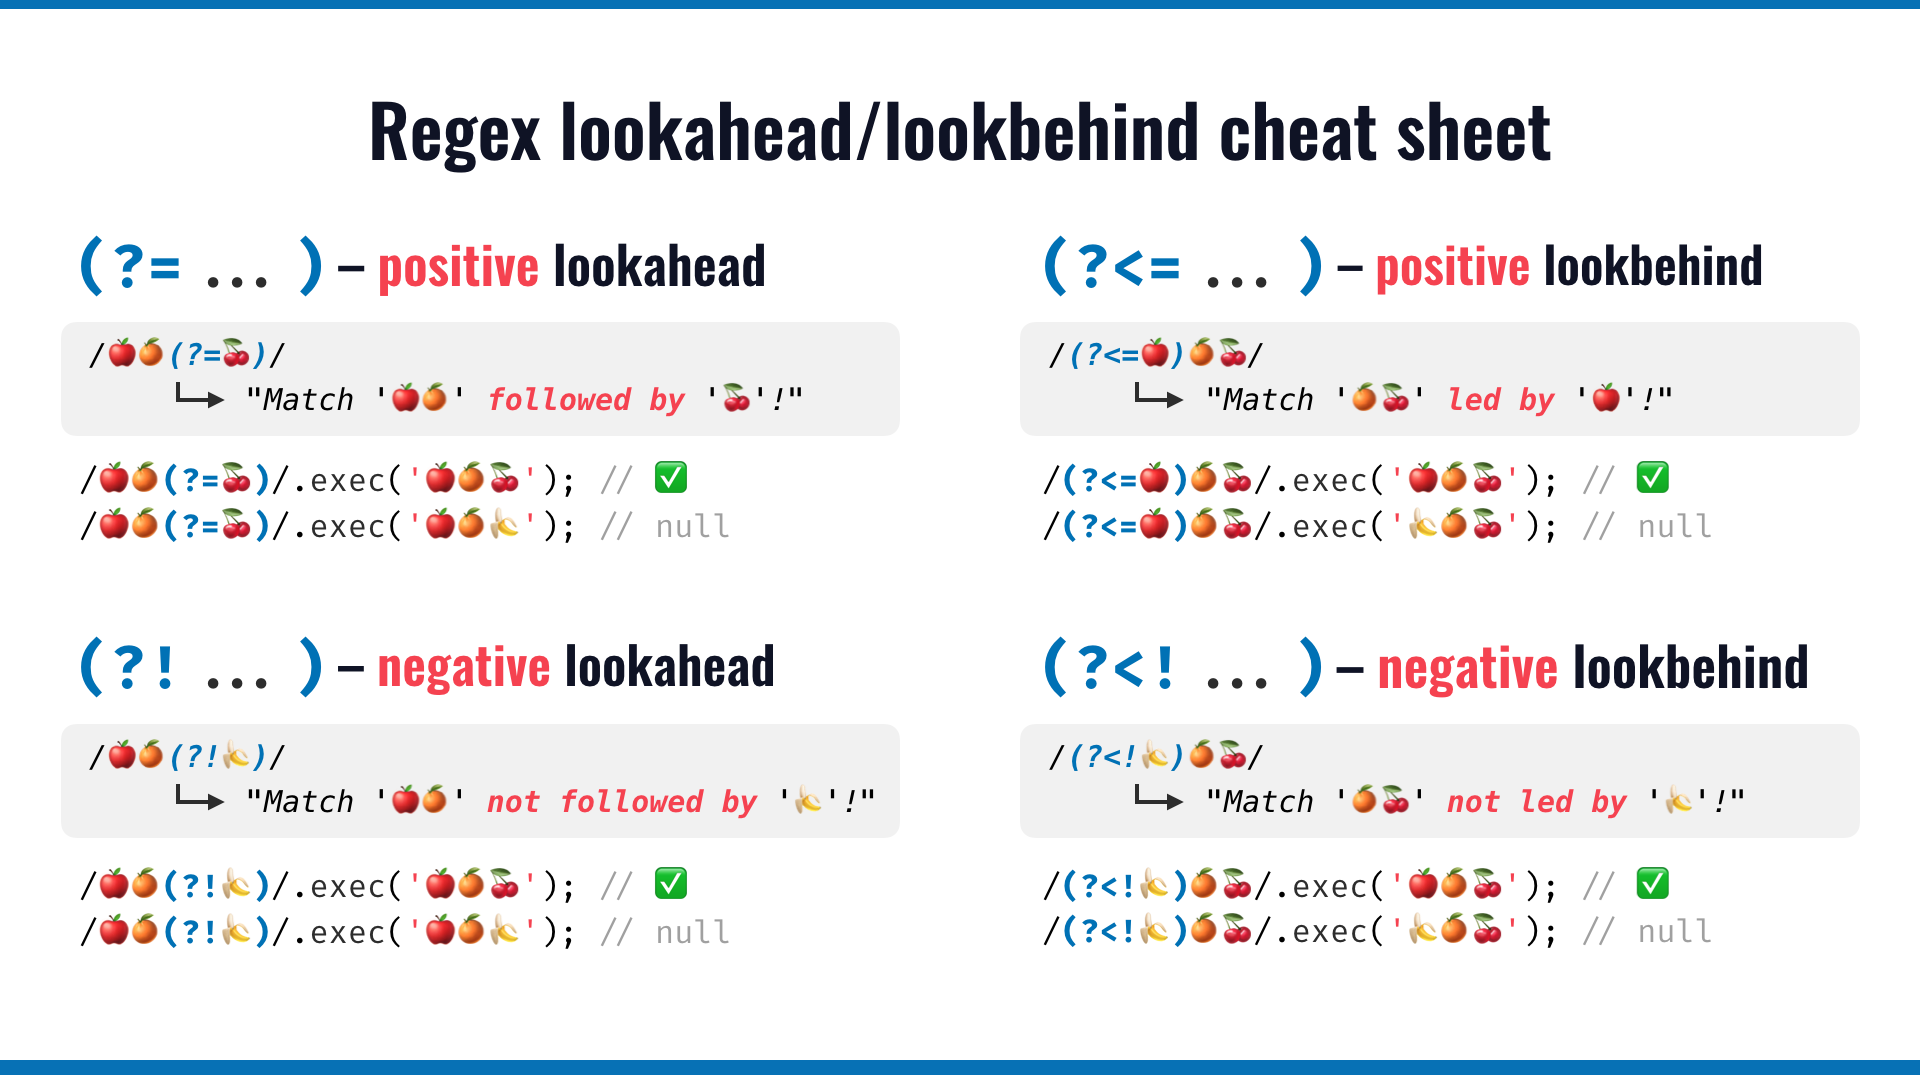
\includegraphics{pcre-look}
  \caption{Positive and Negative Look-ahead and look-behind assertions}
  \labfig{pcre-look}
\end{figure}

\subsection{Comments}

A comment begins with \lstinline|(?#| and ends at the next closing parenthesis.

\subsection{Recursive patterns}

A pattern can refer back to itself recursively or to any subpattern. For example, the pattern \lstinline:\((a*|(?R))*\): will match any combination of balanced parentheses and "a"s.

\newpage
\section{Other Text Processing Tools}

Now that we have discussed the basics of regular expressions, let us see how we can use them in some text processing utilities. We will discuss the following text processing utilities:

\begin{itemize}
  \item \lstinline|tr| - Translate characters.
  \item \lstinline|cut| - Cut out fields (columns) from a line.
  \item \lstinline|grep| - Search for patterns in a file.
  \item \lstinline|sed| - Stream editor - search and replace, insert, select, delete, translate.
  \item \lstinline|awk| - A programming language for text processing.
\end{itemize}

However, these are not all the text processing tools that exist. There are many other text processing utilities that are used in Unix-like systems. Some of them are:

\begin{itemize}
  \item \lstinline|rg| - ripgrep - A search tool that combines the usability of The Silver Searcher (ag) with the raw speed of grep. Useful to find files recursively in a directory or git repository.
  \item \lstinline|fzf| - Fuzzy Finder - A command-line fuzzy finder. Useful to search for files and directories even when you might not know a valid substring of the text. It works by searching for subsequences instead of substrings and other fuzzy search logic. It is extremely powerful when paired with other applications as an interactive select menu.
  \item \lstinline|csvlens| - A tool to view and query CSV files. It is useful to view and query CSV files in a tabular format. It can search for data in a CSV using regex.
  \item \lstinline|pdfgrep| - A tool to search for text in PDF files. It is useful to search for text in PDF files. It can search for text in a PDF using regex. It also supports PCRE2.
\end{itemize}

There are other useful utilities which are not part of GNU coreutils, but are very useful in text processing. Feel free to find such tools, install them, and play around with them. However, we wont be able to discuss those in detail here.

\subsection{tr}

\lstinline|tr| is a command that is used to translate characters. It is used to replace characters in a string with other characters. It is useful when we want to replace a list of characters with another list of characters, or remove a character from a string. It is trivial to create rotation ciphers using \lstinline|tr|.

Without any flags, \lstinline|tr| takes two arguments, \lstinline|LIST1| and \lstinline|LIST2|, which are the two list of characters. \lstinline|LIST1| is the source map and \lstinline|LIST2| is the destination map of the translation. A character can only map to a single character in a translation, however multiple character can map to the same character. That is, it can be many-to-one, but not one-to-many.

\begin{marginfigure}
  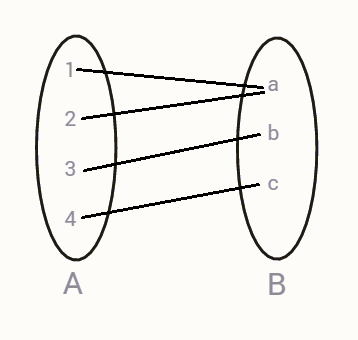
\includegraphics{many-to-one}
  \caption{Many-to-one mapping}
  \labfig{many-to-one}
\end{marginfigure}

A simple example of \lstinline|tr| is to convert a single character to another character.

\begin{lstlisting}
$ echo "hello how are you" | tr 'o' 'e'
helle hew are yeu
\end{lstlisting}

However, the true power of \lstinline|tr| is when we use character lists. We can use character lists to replace multiple characters with other characters.

\begin{lstlisting}
$ echo "hello how are you" | tr 'a-z' 'A-Z'
HELLO HOW ARE YOU
\end{lstlisting}

\lstinline|tr| can also toggle case of characters, that is, the \lstinline|LIST1| and \lstinline|LIST2| can have common characters.

\begin{lstlisting}[language=bash]
$ echo "Hello How Are You" | tr 'a-zA-Z' 'A-Za-z'
hELLO hOW aRE yOU
\end{lstlisting}

We do not need to surround the character ranges in brackets.

\subsubsection{Ciphers}

\begin{definition}[Cipher]
  A cipher is an algorithm for performing encryption or decryption—a series of well-defined steps that can be followed as a procedure. An alternative, less common term is encipherment. To encipher or encode is to convert information into cipher or code. In cryptography, encryption is the process of encoding information. This process converts the original representation of the information, known as plaintext, into an alternative form known as ciphertext. Ideally, only authorized parties can decipher a ciphertext back to plaintext and access the original information.
\end{definition}

One of the common ciphers are rotation ciphers, where each character is replaced by another character that is a fixed number of positions down the alphabet. This is also known as the Caesar cipher, named after Julius Caesar, who is said to have used it to communicate with his generals.

\begin{marginfigure}
  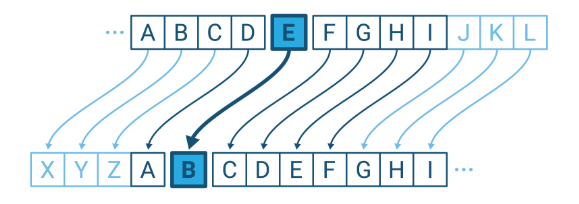
\includegraphics{caesar}
  \caption{Caesar Cipher}
  \labfig{caesar}
\end{marginfigure}

If the shift is 13
\sidenote{
  This is special because the shift of 13 is the same for both encoding and decoding. This is because the English alphabet has 26 characters, and 13 is half of 26. Thus, if we shift by 13, we will get the same character when we shift back by 13.
  It is thus an involution, that is, applying it twice will give the original text.
}
then the cipher is called ROT13. It is a simple letter substitution cipher that replaces a letter with the 13th letter after it in the alphabet. ROT13 is a special case of the Caesar cipher which was developed in ancient Rome.

Let us try to implement ROT13 using \lstinline|tr|.

\begin{lstlisting}[language=bash]
$ echo "hello how are you?" | tr 'a-zA-Z' 'n-za-mN-ZA-M'
uryyb ubj ner lbh?
$ echo "uryyb ubj ner lbh?" | tr 'a-zA-Z' 'n-za-mN-ZA-M'
hello how are you?
\end{lstlisting}

Observe how running the output of the cipher through the same cipher gives us back the original plain-text. This is because ROT13 is an involution cipher.

We can concatenate multiple ranges of characters in the character-lists as seen above, \lstinline|tr| simply converts each character in \lstinline|LIST1| to its corresponding character in \lstinline|LIST2|. The length of both the lists should thus be same. However, if the \lstinline|LIST2| is smaller than \lstinline|LIST1|, \lstinline|tr| will simply repeat the last character of \lstinline|LIST2| as many times as required to make both the lists same length.

\begin{lstlisting}[language=bash]
$ echo "abcdefghijklmnopqrstuvwxyz" | tr 'a-z' '1'
11111111111111111111111111
$ echo "abcdefghijklmnopqrstuvwxyz" | tr 'a-z' '12'
12222222222222222222222222
$ echo "abcdefghijklmnopqrstuvwxyz" | tr 'a-z' '123'
12333333333333333333333333
$ echo "abcdefghijklmnopqrstuvwxyz" | tr 'a-z' '1234-9'
12345678999999999999999999
\end{lstlisting}

The characters in the list are treated as characters, and not digits, thus we cannot replace a character with a multi-digit number. the range \lstinline|1-26| will not result to $26$ numbers from $1$ to $26$, rather, it results in three numbers: $1$, $2$, and $6$. Similarly \lstinline|1-72| means $1,2,3,4,5,6,7,2$.

\begin{lstlisting}[language=bash]
$ echo "abcdefghijklmnopqrstuvwxyz" | tr 'a-z' '1-26'
12666666666666666666666666
$  tr 'a-z' '1-72' <<< "abcdefghijklmnopqrstuvwxyz"
12345672222222222222222222
\end{lstlisting}

We can also repeat a character any arbritrary number of times by using the \lstinline|*| character in the \lstinline|LIST2| inside square brackets.

\begin{lstlisting}[language=bash]
$ echo "abcdefghijklmnopqrstuvwxyz" | tr 'a-z' '1-4[5*10]7'
12345555555555777777777777
\end{lstlisting}

Here the repeat number is actually treated as a number, and thus multi-digit numbers (as shown above) can be used to repeat the character any number of times.

\lstinline|tr| can perform any cipher that does not depend on additional memory or state.

\subsubsection{Deletion}

\lstinline|tr| can also delete or drop characters from a string of characters.
The flag \lstinline|-d| is used to delete characters from the input string.
The syntax is \lstinline|ls -d 'LIST1'|, where \lstinline|LIST1| is the list of characters to delete.

\begin{lstlisting}[language=bash]
$ echo "hi! hello how are you?" | tr -d 'aeiou'
h! hll hw r y?
\end{lstlisting}

Here we are deleting all the vowels from the input string.

We can also use ranges to delete characters.

\begin{lstlisting}[language=bash]
$ echo "hi! hello how are you?" | tr -d 'a-m'
! o ow r you?
\end{lstlisting}

Here we are deleting all the characters from \lstinline|a| to \lstinline|m|.

Sometimes the characters we want to delete is a lot, and its easier to specify the characters we want to keep. We can use the \lstinline|-c| flag to complement the character list, that is, to keep the characters that are in the list.

\begin{lstlisting}[language=bash]
$ echo "hi! hello how are you?" | tr -cd 'a-m'
hihellhae
\end{lstlisting}

Here we are keeping only the characters from \lstinline|a| to \lstinline|m|.
Observe that it also deletes the punctuations, spaces and the newline characters
as well.

This is useful if we want to filter out only some characters from a stream of random characters, for example when trying to generate a random
\sidenote{
  It is not recommended to use \lstinline|/dev/random| instead of \lstinline|/dev/urandom| as it will block if there is a lack of enough entropy. We should totally avoid using \lstinline|RANDOM| variable for cryptographic works since it is not cryptographically secure random number. Computers cannot really generate random numbers, since they are deterministic. Most random number generators simply use external variables like the voltage, temperature, and microphone noise to simulate randomness. This may seem random to humans but is not cryptographically secure for use in generating passwords. There are more secure algorithms to generate passwords. Read more about it
  \href{https://en.wikipedia.org/wiki/Cryptographically\_secure\_pseudorandom\_number\_generator}{here}.
}
password.

\begin{lstlisting}[language=bash]
$ tr -cd 'a-zA-Z0-9' < /dev/urandom | head -c 20 ; echo
8JOzmr4BUbho6wDPaipT
\end{lstlisting}

This uses the \lstinline|/dev/urandom| file to generate random characters, and then filters out only the alphanumeric characters. The \lstinline|head -c 20| is used to print only the first 20 characters, and the \lstinline|echo| is used to print a newline after the password.

\subsubsection{Squeeze}

Finally, \lstinline|tr| can also be used to squeeze characters, that is, to replace multiple consequtive occurrences of a character with a single occurrence. The \lstinline|-s| flag is used to squeeze characters.
It also takes a single argument, which is the list of characters to squeeze.

\marginnote{
  Use single quotes for this example, and not double quotes, as \lstinline|!!| has special meaning in double quotes. It expands to the last run command. This is useful when you write a long command and forget to use \lstinline|sudo|, instead of typing the entire thing again, or using arrow keys, simply type \lstinline|sudo !!| to expand the \lstinline|!!| with the entire previous command.
}
\begin{lstlisting}[language=bash]
$ echo 'Hello!!!!! Using multiple punctuations is not only gramatticaly incorrect but also obnoxious!' | tr -s '!'
Hello! Using multiple punctuations is not only gramatticaly incorrect but also obnoxious!
\end{lstlisting}

\subsection{cut}

If you want to extract a certain column, or a certain range of columns
from a structured text file, doing so using regular expressions can be
a bit cumbersome.

\marginnote{
 Lets try to parse the PCRE regex \lstinline|[^,]*,\\K[^,]*(?=,[^,]*)| to extract the second column from a CSV file. \\ \\
 The first part, \lstinline|[^,]*,| matches the first column, and the \lstinline|\\K| is used to reset the start of the match. This ensures that the first column is present, but not matched and thus not printed.\\ \\
 The second part, \lstinline|[^,]*| matches the second column.
 We are matching as many non-comma characters as possible.\\ \\
 The \lstinline|(?=,[^,]*)| is a lookahead assertion, and is used to match the third column. This ensures that it matches only the second column, and no other column. It will ensure a third column is present, but not match it, thus not printing it. \\ \\
 We had to use \lstinline|\\K| and we could not use a lookbehind assertion, as lookbehind assertions are fixed length, and we do not know the length of the first column. We could have used a lookbehind assertion if we knew the length of the first column.
}
\begin{lstlisting}[language=bash]
$ cat data.csv
name,age,gender
Alice,18,F
Bob,32,M
Carla,23,F
$ grep -P '[^,]*,\K[^,]*(?=,[^,]*)' data.csv -o
age
18
32
23
\end{lstlisting}

As seen above, we can use regular expressions to extract the second column from a CSV file. However, this is not very readable, and can be cumbersome for large files with a lot of columns. This also requires using PCRE to avoid matching the lookbehind and the lookaheads. However, this can be done in an easier manner. This is where the \lstinline|cut| command comes in.

Using \lstinline|cut|, this operation becomes trivial.

\begin{lstlisting}[language=bash]
$ cat data.csv
name,age,gender
Alice,18,F
Bob,32,M
Carla,23,F
$ cut -d, -f2 data.csv
age
18
32
23
\end{lstlisting}

The \lstinline|-d| flag is used to specify the delimiter, and the \lstinline|-f| flag is used to specify the field. The delimiter is the character that separates the fields, and the field is the column that we want to extract. The fields are numbered starting from 1.

\lstinline|cut| can also extract a range of columns.

\marginnote{
  The range is inclusive, that is, it includes the start and end columns.\\ \\
  If the start of the range is absent, it is assumed to be the first column. \\ \\
  If the end of the range is absent, it is assumed to be the last column. \\ \\
  This lets us extract columns even if we do not know the number of columns in the file.
}
\begin{lstlisting}[language=bash]
$ cat data.csv
name,age,gender
Alice,18,F
Bob,32,M
Carla,23,F
$ cut -d, -f1,3 data.csv
name,gender
Alice,F
Bob,M
Carla,F
$ cut -d, -f2-3 data.csv
age,gender
18,F
32,M
23,F
$ cut -d, -f2- data.csv
age,gender
18,F
32,M
23,F
\end{lstlisting}

We can also mention disjoint sets of columns or ranges of columns separated by commas.

\marginnote{
  Here we are using the \lstinline|/etc/passwd| file as an example. The \lstinline|/etc/passwd| file is a text file that contains information about the users on the system. It contains information like the username, user ID, group ID, home directory, and shell. The file is a colon-separated file, where each line contains information about a single user. The fields are separated by colons, and the fields are the username, password (it is not stored, so it is always x), user ID, group ID, user information (this is usually used by modern distrbutions to store the user's full name), home directory, and shell. The file is readable by all users, but only writable by the root user. The file is used by the system to authenticate users and to store information about the users on the system.
}
\begin{lstlisting}[language=bash]
$ cut -d: -f1,5-7 /etc/passwd | tail -n5
dhcpcd:dhcpcd privilege separation:/:/usr/bin/nologin
redis:Redis in-memory data structure store:/var/lib/redis:/usr/bin/nologin
saned:SANE daemon user:/:/usr/bin/nologin
tor::/var/lib/tor:/usr/bin/nologin
test1::/home/test1:/usr/bin/bash
\end{lstlisting}

\begin{exercise}
  Now that you are familiar with the \lstinline|/etc/passwd| file, try to extract the usernames and the home directories of the users. The usernames are the first field, and the home directories are the sixth field. Use the \lstinline|cut| command to extract the usernames and the home directories of the users.
\end{exercise}

\subsubsection{Delimiter}

The default delimiter for \lstinline|cut| is the tab character. However, we can specify the delimiter using the \lstinline|-d| flag. Although it is not required to quote the delimiter, certain characters might be apprehended by the shell and not passed as-is to the command, hence it is always best practice to quote the delimiter using single-quotes. The delimiter has to be a single character, and cannot be more than one character.

The input delimiter can only be speficied if splitting the file by fields, that is, when we are using \lstinline|-f| flag with a field or range of fields.

\subsubsection{Output Delimiter}

The output delimiter by defalut is the same as the input delimiter. However, we can specify the output delimiter using the \lstinline|--output-delimiter| flag. The output delimiter can be a string, and not just a single character. This is useful when we want to change the delimiter of the output file.

\marginnote{
  \lstinline|cut|, like most coreutils, will read the data from standard input (stdin) if no file is specified. This is useful when we want to pipe the output of another command to \lstinline|cut|.
}
\begin{lstlisting}[language=bash]
$ head -n1 /etc/passwd | cut -d: -f5- --output-delimiter=,
root,/root,/usr/bin/bash
$ head -n1 /etc/passwd | cut -d: -f5- --output-delimiter=,,
root,,/root,,/usr/bin/bash
\end{lstlisting}

\subsubsection{Character Range}

The \lstinline|-b| flag is used to extract bytes from a file. The bytes are numbered starting from 1. The byte range is inclusive, that is, it includes the start and end bytes. If the start of the range is absent, it is assumed to be the first byte. If the end of the range is absent, it is assumed to be the last byte.

If we are working with a file with multi-byte characters, the \lstinline|-b| flag will not work as expected, as it will extract bytes, and not characters.
Then we can use the \lstinline|-c| flag to extract characters from a file. The characters are numbered starting from 1. However, in GNU cut, the feature is not yet implemented. If you are using \textbf{freebsd cut} then the difference can be observed.

\begin{lstlisting}[language=bash]
$ head -n1 /etc/passwd | cut -b5-10
:x:0:0
$ head -n1 /etc/passwd | cut -c5-10
:x:0:0
\end{lstlisting}

\subsubsection{Complement}

Sometimes its easier to specify the fields we want to drop, rather than the fields we want to keep. We can use the \lstinline|--complement| flag to drop the fields we specify.

Recall that the second field of the \lstinline|/etc/passwd| file is the password field, which is always \lstinline|x|. We can drop this field using the \lstinline|--complement| flag.

\begin{lstlisting}[language=bash]
$ head -n1 /etc/passwd
root:x:0:0:root:/root:/usr/bin/bash
$ head -n1 /etc/passwd | cut -d: --complement -f2
root:0:0:root:/root:/usr/bin/bash
\end{lstlisting}

\subsubsection{Only Delimited Lines}

Sometimes we have a semi-structured file, where some lines are delimited by a character, and some are not. We can use the \lstinline|--only-delimited| flag to print only the lines that are delimited by the delimiter.

\marginnote{
  Note that if we mention a field number that is not present in the line, \lstinline|cut| will simply print nothing. If we print fields 1 to 3, and there are only 2 fields, it will print only first two fields, etc.
}
\begin{lstlisting}[language=bash]
$ cat data.csv
name,age,gender
Alice,18,F
Bob,32,M
Carla,23,F
# This is a comment
$ cut -d, -f1,3 data.csv
name,gender
Alice,F
Bob,M
Carla,F
# This is a comment
$ cut -d, -f1,3 data.csv  --only-delimited
name,gender
Alice,F
Bob,M
Carla,F
\end{lstlisting}

Cut is a very handy tool for text processing, we will be using it extensively in the upcoming chapters.

\subsection{paste}

\lstinline|paste| is a very simple command that is used to merge lines of files.
It is used to merge lines of files horizontally, that is, to merge lines from multiple files into a single line. It is useful when we want to merge lines from multiple files into a single line, and separate them by a delimiter. It can also be used to join one file into a single line separated by a delimiter.

\begin{lstlisting}[language=bash]
$ cat file1.txt
hello world
this is file1
$ cat file2.txt
this is file2
and it has more lines
than file1
$ paste file1.txt file2.txt
hello world     this is file2
this is file1   and it has more lines
        than file1
\end{lstlisting}

The default delimiter is the tab character, however we can specify the delimiter using the \lstinline|-d| flag.

\begin{lstlisting}[language=bash]
$ paste -d: file1.txt file2.txt
hello world:this is file2
this is file1:and it has more lines
:than file1
\end{lstlisting}

Paste can also be used to merge lines from a single file into a single line.
The \lstinline|-s| flag is used to merge lines from a single file into a single line.
We can specify the delimiter for this as well using the \lstinline|-d| flag.

\begin{lstlisting}[language=bash]
$ paste -d: -s file1.txt
hello world:this is file1
\end{lstlisting}

This is better than using \lstinline|tr '\n' ':'| to replace the newline character with a delimiter, as \lstinline|tr| will also replace the last newline character of the last line, giving a trailing delimiter.

\begin{lstlisting}[language=bash]
$ tr '\n' ':' < file1.txt
hello world:this is file1:
\end{lstlisting}

This is very helpful when we want to find the sum of numbers in a file.

\begin{lstlisting}[language=bash]
$ cat numbers.txt
1
4
2
6
7
2
$ paste -sd+ numbers.txt
1+4+2+6+7+2
$ paste -sd+ numbers.txt | bc
22
\end{lstlisting}

Here we are first using \lstinline|paste| to merge the lines of the file into a single line, separated by the \lstinline|+| character. We then pipe this to \lstinline|bc|, which is a command line calculator, to calculate the sum of the numbers.

\subsection{fold}

Just like we can use \lstinline|paste| to merge lines of a file, we can use \lstinline|fold| to split lines of a file. \lstinline|fold| is a command that is used to wrap lines of a file. It is used to wrap lines of a file to a specified width.

\begin{lstlisting}[language=bash]
$ cat data.txt
123456789
$ fold -w1 data.txt
1
2
3
4
5
6
7
8
9
$ fold -w2 data.txt
12
34
56
78
9
\end{lstlisting}

We can also force \lstinline|fold| to break lines at spaces only, and not in the middle of a word. However, if it is not possible to maintain the maximum width specified if breaking solely on spaces, it will break on non-spaces as well.

\begin{lstlisting}[language=bash]
$ cat text.txt
This is a big block of text
some of these lines can break easily
Whereas_some_are_to_long_to_break
$ fold -sw10 text.txt
This is a
big block
of text
some of
these
lines can
break
easily
Whereas_so
me_are_to_
long_to_br
eak
\end{lstlisting}

This is useful if you want to undo the operation of \lstinline|tr -d '\n'| performed on lines of equal width.

\subsection{grep}

\lstinline|grep| is a command that is used to search for patterns in a file. It is used to search for a pattern in a file, and print the lines that match the pattern.

Grep has a lot of flags and features, and is a very powerful tool for searching for patterns in a file.
It can search using \textbf{BRE}, \textbf{ERE}, and even \textbf{PCRE}.

We will discuss \lstinline|grep| in detail in the next chapter.

\subsection{sed}

\lstinline|sed| is a stream editor that is used to perform basic text transformations on an input stream. It is used to search and replace, insert, select, delete, and translate text.

Sed is a sysadmin's go to tool for perform quick text transformations on files.
It can also perform the changes directly on the file, without needing to write the changes to a new file.

We cover \lstinline|sed| in detail in later chapters.

\subsection{awk}

\lstinline|awk| is a programming language that is used for text processing and data extraction. It is a very powerful tool for text processing, and is used to extract and manipulate data from files.

It has its own programming language, although with very few keywords, and is very easy to learn.

We cover \lstinline|awk| in detail in later chapters.
